\documentclass[11pt]{article}
\usepackage[a4paper,margin=1in]{geometry}
\usepackage{amsmath,amssymb,amsthm,mathtools}
\usepackage{booktabs}
\usepackage{enumitem}
\usepackage{float}
\usepackage{graphicx}
\usepackage{hyperref}
\usepackage[nameinlink,capitalise]{cleveref}
\usepackage[numbers,sort&compress]{natbib}

\newtheorem{theorem}{Theorem}[section]
\newtheorem{proposition}[theorem]{Proposition}
\newtheorem{remark}[theorem]{Remark}
\newcommand{\norm}[1]{\left\lVert#1\right\rVert}

\title{Two Corridors to Stage A1 and the Conditional Closure of Intrinsic Identification\\
\large Full-Block Scaling, Effective-Rank Futures, and the Quarter-Power Exponent Ledger}
\author{Liang Wang}
\date{July 2026}

\begin{document}
\maketitle

\begin{abstract}
RH-75 identified a full-block route to a polylogarithmic small-noise Hardy
bound.  RH-76 ruled out single-arc phase compression, while RH-77 found a
second route: uniformly tiny postblock effective rank.  This paper composes
both alternatives with the earlier intrinsic-identification theorems and
isolates the sole remaining Stage-A premise.

In the full-block corridor, a log-square horizon together with
$\norm{A_k^{M_k}}=O(\sqrt{\sigma_k})$ gives
$E_{B,k},E_{C,k}=\operatorname{polylog}(1/\sigma_k)$.  In the effective-rank
corridor, decompose $A_k^{M_k}X_k=B_{k,r}+R_{k,r}$; if the reduced future and
the observability-transferred residual are polylogarithmic, the same Hardy
conclusion follows.  Either corridor has zero power of $\sigma$.

RH-54's factor-aware theorem then yields
\[
 \norm{I_{n,\sigma}}_{S_2}
 =O\!\left(n^{-2}\sigma^{-13/4}
 \operatorname{polylog}(1/\sigma)\right).
\]
For every strict schedule $n\sigma^2\to\infty$, this tends to zero.  Thus an
all-level proof of either corridor closes Stage A1 and, together with the
already rigorous RH-54/RH-55 transfer, makes the intrinsic identification
unconditional.  No simultaneous proof of both corridors is required.

A 256-bit Arb composition audit checks the five validated anchors.  The common
per-channel Hardy upper grows only from $1.079$ to $1.836$; every frozen Hardy
product lies inside the conditional envelope.  The Hardy sigma-power is zero,
strictly below the quarter-power threshold.  On the stress mesh
$n=\sigma^{-2}(k+2)$, the identification envelope decreases from $0.07355$
to $0.002961$.  RH-77 rank-four future errors remain below
$5.35\times10^{-6}$.

This is a conditional closure theorem, not an all-dyadic proof.  The sole
remaining Stage-A premise is an analytic all-level theorem for at least one
corridor.  Stage A1, unconditional Stage A4, Hilbert--Polya, and the Riemann
Hypothesis remain open.
\end{abstract}

\noindent\textbf{Keywords:} conditional composition; Hardy energy;
effective rank; dyadic mesh; intrinsic Riesz identification.

\medskip
\noindent\textbf{MSC 2020:} 47A10; 47B10; 47B35; 65G20.

\section{Introduction}

The Stage-A route now has a cleaner logical structure than it did at RH-50.
Finite-scale assembly and Hardy completion are rigorous end to end.  Adaptive
strong--weak Riesz transfer is available.  The only missing ingredient is a
uniform directional Hardy budget over the physical dyadic family.

RH-75 gave a sufficient full-operator law \citep{WangScaling2026}.  RH-77 gave
a different, source-specific reduction based on postblock singular values
\citep{WangRank2026}.  The purpose of this paper is to show that these are
alternative corridors into the same downstream theorem.  This matters
because the full Frobenius block law may be harder to prove than directional
rank decay; the program should not require the stronger statement if the
weaker physical one suffices.

\section{Corridor I: full-block scaling}

Let $\sigma_k=\sigma_0 2^{-k}$.  The RH-75 hypotheses give
\[
 M_k=O(k^2),\quad
 \norm{A_k^{M_k}}\le C_q\sqrt{\sigma_k},\quad
 \sigma_k\norm{Y_k}^2\le C_y,
\]
together with polylogarithmic one-block source and finite-prefix energies.
The block theorem then implies
\begin{equation}
 E_k^2\le C_f(k+a)^f+C_t(k+a)^s.
 \label{eq:block-corridor}
\end{equation}
Thus $E_k$ is polylogarithmic and carries no negative power of $\sigma_k$.

\section{Corridor II: effective-rank future}

Let $B_k=A_k^{M_k}X_k$ and choose a rank-$r_k$ approximation
$B_{k,r}$.  Split the Hardy energy into its finite prefix and future.  RH-77
gives
\begin{equation}
 |T_k(B_k)-T_k(B_{k,r})|
 \le G_k^{1/2}\norm{B_k-B_{k,r}}_{S_2},
 \label{eq:rank-error}
\end{equation}
where
$G_k=\norm{O_{k,M_k}}/(1-\norm{A_k^{M_k}}^2)$.

\begin{theorem}[Effective-rank Stage A1 corridor]
\label{thm:rank-corridor}
Suppose the finite prefix, reduced future $T_k(B_{k,r})$, and right side of
\eqref{eq:rank-error} are each polylogarithmic in $1/\sigma_k$.  Then the full
Hardy energy is polylogarithmic.  The rank schedule itself may be fixed or
polylogarithmic.
\end{theorem}

\begin{proof}
Apply the triangle inequality to the finite-prefix/future decomposition and
then \eqref{eq:rank-error}.  A finite sum of polylogarithmic quantities is
polylogarithmic.
\end{proof}

This corridor is strictly directional.  It does not imply a small full-space
operator norm and therefore does not conflict with fixed-depth no-go results.

\section{Composition into intrinsic identification}

RH-54 proved that if
\[
 E_B=O(\sigma^{-\alpha_B}),\qquad
 E_C=O(\sigma^{-\alpha_C}),
\]
and the range-restricted residues are bounded, then
\begin{equation}
 \norm{I_{n,\sigma}}_{S_2}
 =O\!\left(n^{-2}\sigma^{-13/4-\alpha_B-\alpha_C}\right).
 \label{eq:rh54}
\end{equation}
Every strict $n\sigma^2\to\infty$ schedule survives when
$\alpha_B+\alpha_C\le1/4$ \citep{WangFactor2026}.  RH-55 supplies the adaptive
strong--weak Riesz/cutoff transfer needed by that theorem
\citep{WangStrongWeak2026}.

\begin{theorem}[Two-corridor conditional Stage A1/A4 closure]
\label{thm:composition}
Assume the already established RH-54/RH-55 residue and transfer hypotheses.
If either the full-block corridor \eqref{eq:block-corridor} or the effective-
rank corridor of \cref{thm:rank-corridor} holds at every dyadic level for both
left and right channels, then:
\begin{enumerate}[label=(\roman*),leftmargin=2.2em]
 \item Stage A1 has a polylogarithmic directional Hardy budget;
 \item $\alpha_B=\alpha_C=0$, so the RH-54 quarter-power gate is strict;
 \item for every schedule $n\sigma^2\to\infty$,
 \begin{equation}
  \norm{I_{n,\sigma}}_{S_2}
  =O\!\left(n^{-2}\sigma^{-13/4}
  \operatorname{polylog}(1/\sigma)\right)\longrightarrow0.
  \label{eq:identification}
 \end{equation}
\end{enumerate}
\end{theorem}

\begin{proof}
Either corridor gives polylogarithmic $E_B,E_C$, hence zero sigma powers.
Insert them into \eqref{eq:rh54}.  Write
$n=\sigma^{-2}L(\sigma)$ with $L(\sigma)\to\infty$; the right side of
\eqref{eq:identification} becomes
$O(\sigma^{3/4}L(\sigma)^{-2}\operatorname{polylog}(1/\sigma))$, which tends
to zero.
\end{proof}

The theorem is a logical closure: it identifies a single missing family
premise, but does not assert that premise.

\section{Five-anchor composition audit}

The RH-75 common constants give
\begin{equation}
 E_{B,k}^2,E_{C,k}^2
 \le0.552(k+2)+0.058788.
 \label{eq:anchor-envelope}
\end{equation}
The audit evaluates this and the RH-54 expression at 256-bit Arb precision
\citep{Johansson2017}.  Every RH-70 frozen product is enclosed by
\eqref{eq:anchor-envelope}.

\begin{table}[H]
\centering
\small
\caption{Conditional common Hardy upper, product upper, rank-four future
error, and identification envelope on $n=\sigma^{-2}(k+2)$.}
\label{tab:audit}
\begin{tabular}{@{}rrrrr@{}}
\toprule
$\sigma$ & Hardy & product & rank-4 error & identification\\
\midrule
0.16 & 1.079 & 1.163 & $5.05\,10^{-9}$ & 0.07355\\
0.08 & 1.310 & 1.715 & $3.40\,10^{-9}$ & 0.02867\\
0.04 & 1.506 & 2.267 & $3.48\,10^{-8}$ & 0.01268\\
0.02 & 1.679 & 2.819 & $6.77\,10^{-10}$ & 0.005997\\
0.01 & 1.836 & 3.371 & $5.35\,10^{-6}$ & 0.002961\\
\bottomrule
\end{tabular}
\end{table}

The anchor envelope has logarithmic energy-squared growth, so both Hardy
sigma powers are zero.  The effective-rank residual is much smaller than the
common energy budget.  The stress identification envelope decreases at every
stored level.

\begin{figure}[H]
\centering
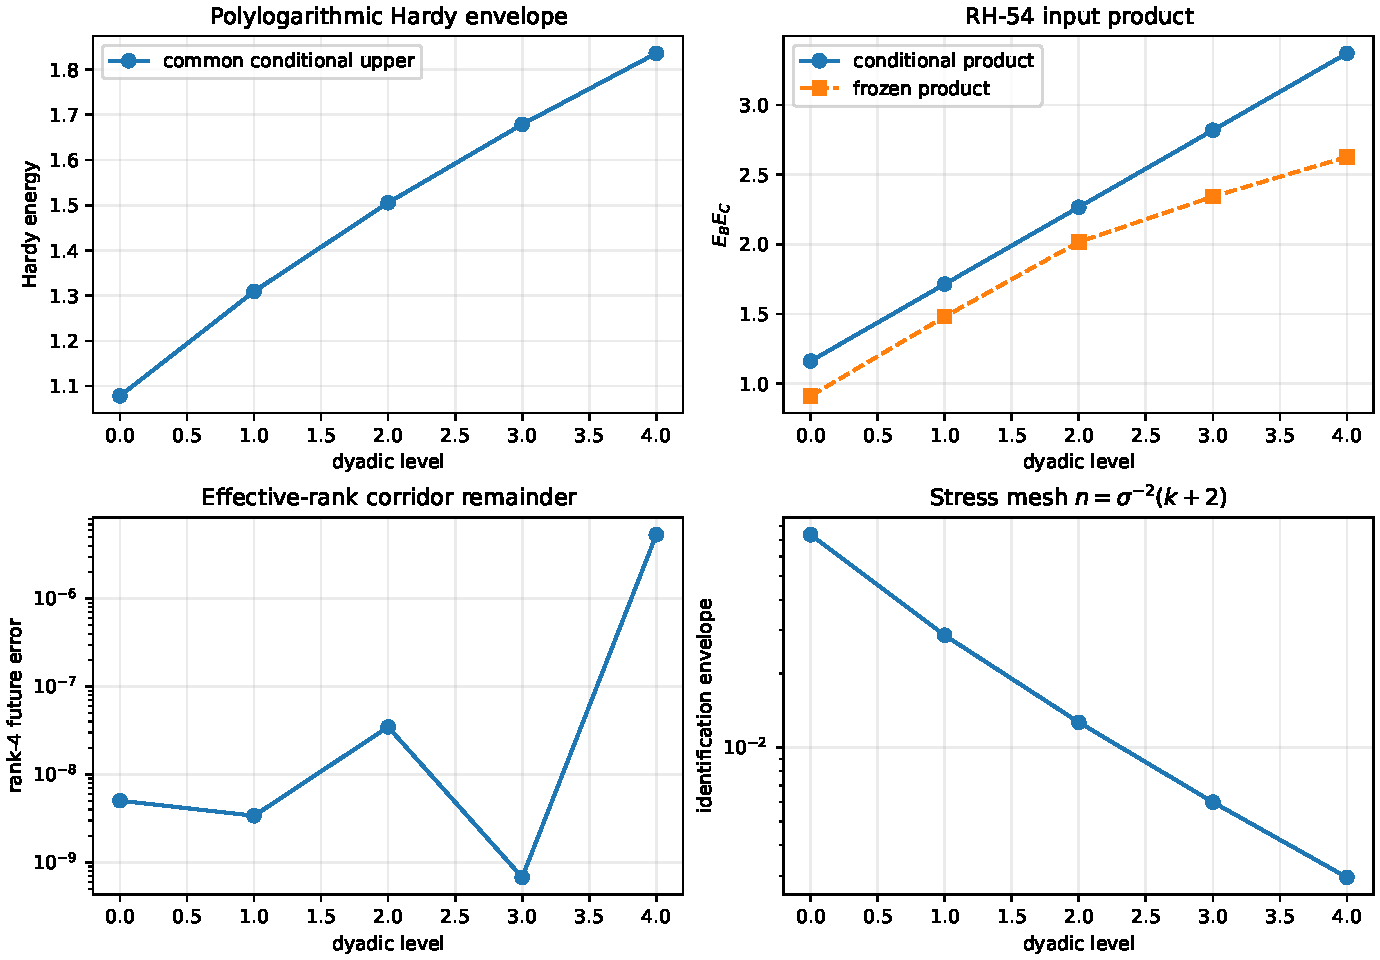
\includegraphics[width=0.98\textwidth]{figures/two_corridor_stage_A1_composition.pdf}
\caption{Conditional Hardy envelope, actual product inclusion, rank-four
remainder, and strict-mesh identification decay.}
\label{fig:audit}
\end{figure}

\section{Exact remaining frontier}

After RH-72--RH-78, the Stage-A dependency graph is:
\[
 \boxed{\text{all-level block law}}
 \quad\text{or}\quad
 \boxed{\text{all-level effective-rank law}}
 \Longrightarrow
 \text{Stage A1}
 \Longrightarrow
 \text{intrinsic identification}.
\]
Finite-scale inclusion, normalized factors, terminal Hardy arithmetic,
adaptive cutoff transfer, and downstream exponent composition are no longer
open in their stated scopes.

RH-79 will examine how this conditional identification feeds the Stage-A4
intrinsic determinant statement and precisely which limit interchanges remain.
The present paper does not prove either all-level premise, so Stage A1 and
unconditional Stage A4 remain open.  It constructs no renormalized determinant
limit, Hilbert--Polya operator, $T\log T$ law, prime-power trace formula,
zeta-zero identity, or proof of the Riemann Hypothesis.

\section{Conclusion}

The route no longer depends on rescuing a failed phase-arc picture.  There are
two mathematically sufficient corridors, and the effective-rank corridor is
strongly supported at the five validated scales.  Proving one all-level
corridor is now the sole Stage-A analytic wall.

\bibliographystyle{plainnat}
\bibliography{references}
\end{document}
